\begin{surferPage}{Eine Cuspe ($A_2^{+-}$ Singularität)}
Eine Cuspen-Singularität einer Fläche erhält man mit der
    Gleichung 
    \vspace*{-0.4em}
    \begin{center}
      $x^3+y^2-z^2=0.$
    \end{center}
    \vspace*{-0.4em}
    Dies ist die flächige Variante einer ebenen Cuspe, die man erhält, wenn
    man die Fläche mit einer geeigneten Ebene schneidet: z.B.\ liefert $z=0$
    die Ebene Kurve $x^3+y^2=0$:
    \vspace*{-0.7em}
    \begin{center}
      \begin{tabular}{c@{\ }c@{\ }c@{\ }c}
        \begin{tabular}{@{}c@{}}
          
\includegraphics[width=1.2cm]{../../common/images/A2pm}
        \end{tabular}
        &
        \begin{tabular}{@{}c@{}}
          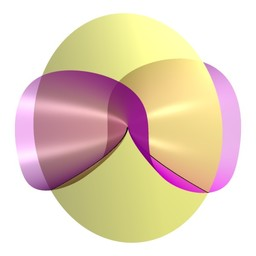
\includegraphics[width=1.2cm]{../../common/images/cuspe_cut}
        \end{tabular}
        &
        \begin{tabular}{@{}c@{}}
          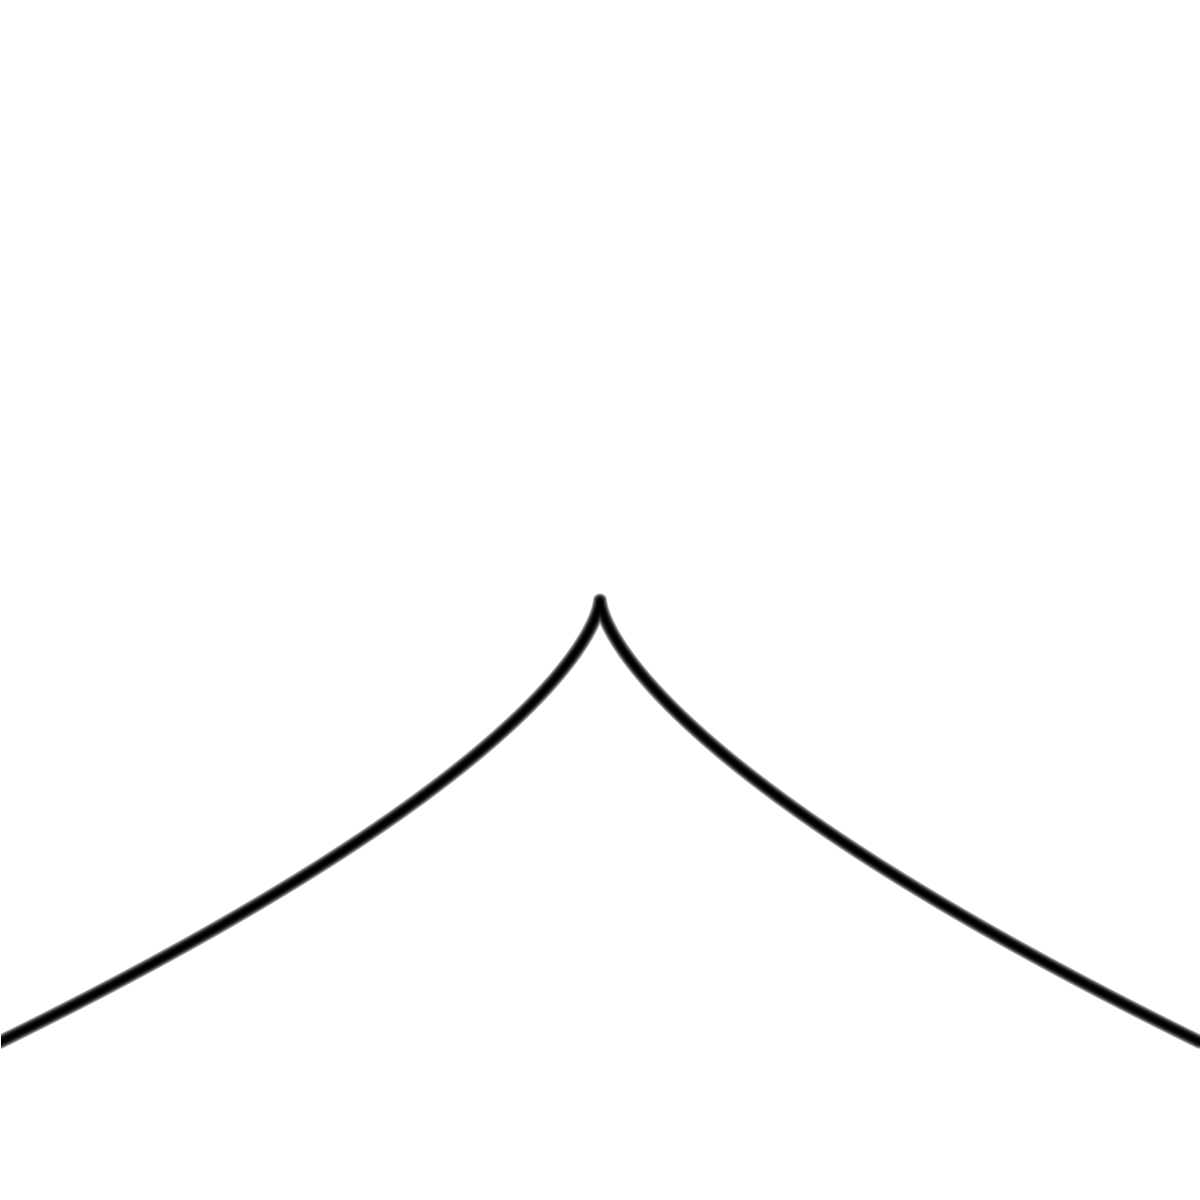
\includegraphics[width=1.2cm]{../../common/images/cuspe_rot}
        \end{tabular}
        &
        \begin{tabular}{@{}c@{}}
          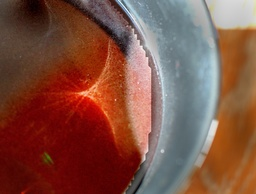
\includegraphics[width=1.4cm]{../../common/images/kuspe_detail_gross_heller}
        \end{tabular}
      \end{tabular}
    \end{center}
    \vspace*{-0.4em}
    Eine Cuspe entsteht auch, wenn Licht in eine Tasse
    Kaffee fällt (rechtes Bild)!

    Man kann eine 
    Singularität vom Typ $A_k^{+-}$ so stören, dass
    $\lfloor\frac{k+1}{2}\rfloor$ Doppelkegel - 
    Singularitäten entstehen, ohne den Grad der Fläche zu erhöhen. 
    Das kann man hier ($k=2$) an der Gleichung der Flächen - Singularität
    leicht sehen: 
    \[(1-a)x^3+ax^2+y^2-z^2=0.\]
    Für $a=0$ findet man eine Cuspe, für $a=1$ den Doppelkegel: 
    \vspace*{-0.6em}
    \begin{center}
      \begin{tabular}{@{}c@{\quad}c@{\quad}c@{}}
        \begin{tabular}{@{}c@{}}
          
\includegraphics[width=1.1cm]{../../common/images/A2pm_0}
        \end{tabular}
        &
        \begin{tabular}{@{}c@{}}
          
\includegraphics[width=1.1cm]{../../common/images/A2pm_1}
        \end{tabular}
        &
        \begin{tabular}{@{}c@{}}
          
\includegraphics[width=1.1cm]{../../common/images/A2pm_2}
        \end{tabular}
      \end{tabular}
    \end{center}
 
\end{surferPage}
